\documentclass[a4paper,12pt]{article}
\usepackage[utf8]{inputenc}
\usepackage[T1]{fontenc}
\usepackage[french]{babel}
\usepackage{geometry}
\geometry{left=2.5cm, right=2.5cm, top=3cm, bottom=3cm}
\usepackage{hyperref}
\usepackage{graphicx}
\usepackage{amsmath}
\usepackage{listings}
\usepackage{xcolor}

\title{Rapport Technique \\ Mini-ERP : Gestion Clients, Produits et Factures}
\author{Ton Nom \\ \texttt{ton.email@example.com}}
\date{\today}

% Configuration listings pour le code JavaScript
\lstset{
  language=JavaScript,
  basicstyle=\ttfamily\small,
  keywordstyle=\color{blue},
  commentstyle=\color{gray}\itshape,
  stringstyle=\color{red},
  numbers=left,
  numberstyle=\tiny,
  stepnumber=1,
  numbersep=5pt,
  showspaces=false,
  showstringspaces=false,
  breaklines=true,
  frame=single,
  captionpos=b
}

\begin{document}

\maketitle

\tableofcontents
\newpage

\section{Introduction}

Ce projet Mini-ERP a pour objectif de gérer efficacement les clients, fournisseurs, produits et factures à travers une application backend utilisant Node.js, Express et une base de données SQLite. Le système permet des opérations CRUD via une API REST.

\section{Analyse et Conception}

\subsection{Modèle de données}

Le modèle de données comprend plusieurs entités principales : \texttt{Clients}, \texttt{Fournisseurs}, \texttt{Produits}, \texttt{Factures} et \texttt{Ligne\_facture}. Ces tables sont reliées par des clés étrangères, notamment entre \texttt{Factures} et \texttt{Clients}, ainsi qu'entre \texttt{Ligne\_facture} et \texttt{Factures} et \texttt{Produits}.

\begin{figure}[h!]
  \centering
  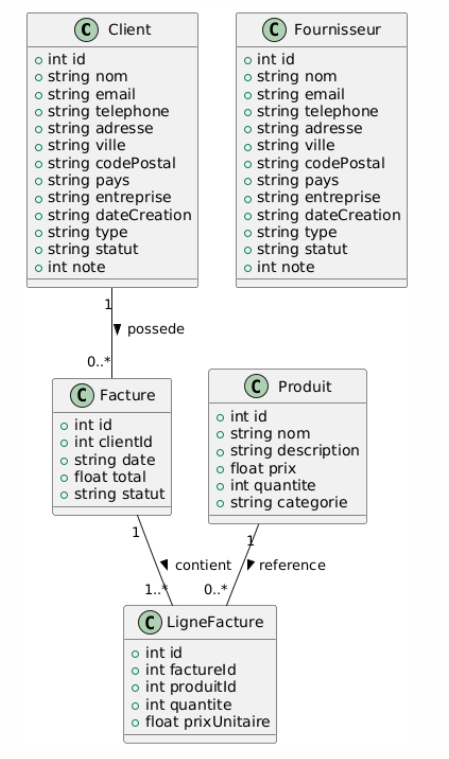
\includegraphics[width=0.85\textwidth]{uml.png}
  \caption{Diagramme de classes UML du Mini-ERP}
  \label{fig:uml}
\end{figure}

\subsection{Architecture}

Le backend est construit avec Node.js et Express pour gérer les requêtes HTTP. La base de données SQLite est utilisée pour stocker les données localement. L'application expose une API REST complète permettant la gestion des entités principales.

\section{Implémentation}

Voici un exemple de route Express pour récupérer la liste des clients :

\begin{lstlisting}[caption=Route GET pour récupérer les clients]
const express = require('express');
const router = express.Router();
const db = require('./db');

router.get('/clients', (req, res) => {
  db.all("SELECT * FROM clients", [], (err, rows) => {
    if (err) {
      return res.status(500).json({error: err.message});
    }
    res.json(rows);
  });
});

module.exports = router;
\end{lstlisting}

La base de données est initialisée avec un script qui crée les tables et insère des données de test.

\section{Tests et Validation}

Des tests manuels ont été réalisés via des requêtes API (Postman, curl). Les données de test permettent de vérifier les relations entre les entités. Voici une capture d’écran de l’outil Postman exécutant une requête GET sur \texttt{/api/clients} :

\section{Conclusion et Perspectives}

Ce projet Mini-ERP répond aux besoins basiques de gestion administrative. Pour aller plus loin, il serait intéressant d’ajouter un frontend React, une authentification utilisateur, et des fonctionnalités avancées comme la gestion des stocks en temps réel.

\appendix
\section{Extrait de code - Script de réinitialisation de la base}

\begin{lstlisting}[caption=reset_db.js]
const sqlite3 = require('sqlite3').verbose();
const db = new sqlite3.Database('./erp.sqlite');

db.serialize(() => {
  db.run("DELETE FROM ligne_facture");
  db.run("DELETE FROM factures");
  db.run("DELETE FROM produits");
  db.run("DELETE FROM clients");
  db.run("DELETE FROM fournisseurs");
  // Reset autoincrement counters...
  // Insert test data...
});
db.close();
\end{lstlisting}

\end{document}
